\section{Introdução}
\begin{frame}{Introdução}
	\begin{block}{Exigências do mercado atual}
		\begin{itemize}
			\item Utilização efetiva de máquinas multi-core por programas concorrentes. 
			\item Criação de aplicações distribuídas voltadas para a Web ou para a Internet.
		\end{itemize}
	\end{block}
\end{frame}

\begin{frame}{Introdução}
    \begin{block}{Linguagens}
        \begin{center}
	        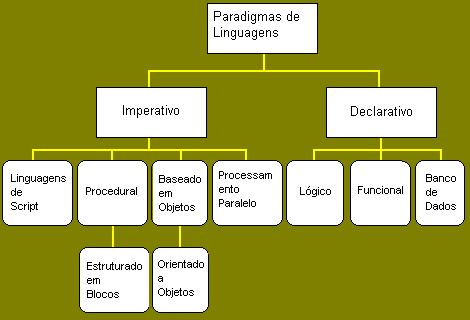
\includegraphics[scale=0.4]{paradigmas-imagem.png} 
        \end{center}
    \end{block}
\end{frame}

\begin{frame}{Introdução}
	\begin{block}{Programação orientada a objetos}
		\begin{itemize}
			\item Estilo imperativo 
			\item Tenta simular o mundo real
			\item A computação é realizada em termos de estados e expressões que podem
			mudar o estado do programa.
		\end{itemize}
	\end{block}
	\begin{center}
		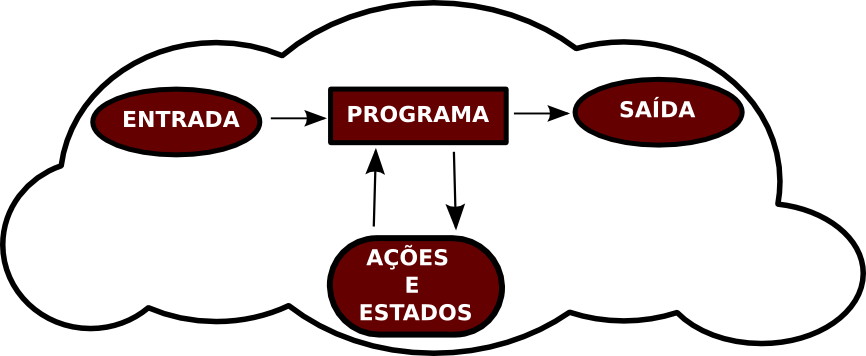
\includegraphics[scale=0.3]{progImp.png}
	\end{center}
\end{frame}

\begin{frame}{Introdução}
	\begin{block}{A Programação Funcional}
		\begin{itemize}
			\item Estilo de programação baseado no uso de funções
			\item Funções são entidades de 1ª classe 
			\item Toda a programação é baseada na avaliação de expressões para gerar valores. 
			\item Cada valor tem um tipo associado.
			\item Funções podem ser nomeadas ou anônimas (lambda)
		\end{itemize}
	\end{block}
\end{frame}

\subsection{Apresentando Scala}
% contextualizar a linguagem
\begin{frame}{Introdução}
	\begin{block}{Scala}
        \begin{itemize}
            \item O nome Scala significa ``linguagem escalável"
            \item Projetada para integrar linguagem orientada a objetos e programação funcional
            \item Executa na JVM
        \end{itemize}
	\end{block}
\end{frame}

\begin{frame}{Scala}
    \begin{block}{Histórico}
        \begin{itemize}
            \item O design começou em 2001 na École Polytechnique Fédérale de Lausanne por Matin Odersky
            \item Primeiro release na plataforma Java: no fim de 2003 e início de 2004 
            \item Versão para plataforma .NET liberada em Junho de 2004
        \end{itemize}
    \end{block}
\end{frame}
%propraganda, doutrinar o povo, enfim igual a java
\subsection{Por que utilizar Scala?}

\begin{frame}{Scala}
    \begin{block}{Por quê utilizar Scala?}
        \begin{itemize}
            \item Linguagem híbrida: simplicidade de funcional + poder de objetos
            \item Fortemente tipada
            \item Linguagem Concisa
            \item Multiplataforma: JVM e .NET 
        \end{itemize}
    \end{block}
\end{frame} 

%motivação tecnica
\subsection{Uma Linguagem Escalável}
